\chapter{Methodology}
\label{chap:met}

\section{SLand Semantic REpresentation Design}
\label{sec:met:ir_design}
Waiting for the SR meeting results

\section{Compiler integration}
\label{sec:met:ls_compiler_interop}
The Language Server idea is to launch the LS instance in the same project directory
opened in the editor, and connect it to the editor via Language Server Protocol.

A Language Server is responsible for language-specific editor features, 
it works on the language Semantic Representation and other metadata 
to perform semantic analysis and consequently provide the editor with usable data in the agreed format via Language Server Protocol.
As Language server heavily relies on the modern compiler, that exposes the SR, 
we need to implement a way to integrate compiler into the Language Server and to enable their interoperation.

There are two possible ways to achieve that: either to use compiler as a library or invoke it in a separate process, 
feeding specific command line arguments.
\begin{table}[H]
    \centering
    \begin{tabular}{|c|c|}
        \hline
        \textbf{invoking as a command} & \textbf{using compiler as a library} \\
        \hline
        simpler integration & harder integration \\ 
        \hline
        very limited invocation options & complex invocation strategies may be expressed \\
        \hline
        need to (de)serialize data & can exchange binary data \\
        \hline
        need to implement IR traversal in the LS & compiler can expose AST traversal API \\
        \hline
        need to describe compiler internal data types in the LS & compiler can expose internal data types \\
        \hline 
    \end{tabular}
    \caption{Compiler integration methods comparison}
    \label{table:met:compiler_integration}
\end{table}

Since the SLang[TODO] compiler does not expose any AST traversal API or internal data types, most of 
the traits specific to an ``integration as a library" option will not be used in our case.
Moreover, the compiler provides a stable json-formatted SR, which being a text-serialized format, 
can be easily transfered via operating system channel like standard output[TODO].

Thus the compiler can be invoked by our Language Server as a command call, we are not limited 
with any functionality that would require ``compiler as a library" traits, and this option
is easier to implement on both Language Server and compiler ends,
therefore we can declare this way of integration the most feasible in our case and stick to it.

\begin{figure}[H]
    \centering
    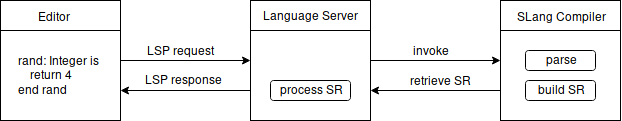
\includegraphics[width=1.0\textwidth]{figs/compiler_integration.png}
    \caption{Workflow with Language Server and integrated compiler}
\end{figure}


\section{Language Server Core Design}
\label{sec:met:ls_design}

\section{Language Server Module System Design}
\label{sec:met:ls_mod}
Description of basic Language Server module system design

\subsection{Code Semantic Based Highlights Design}
\label{sec:met:ls_mod:semhighlight}
Architecture and methods of IR analysis for hightlights

Mapping from semantic entities to LSP highlighting staff

\subsection{Autocomplete Design}
\label{sec:impl:ls_mod:autocomplete}
Description if autocomplete argorithms and data structures choice